\documentclass[10pt,a4paper]{article}

\usepackage[a4paper,top=1.8cm,bottom=1.8cm,left=1.85cm,right=1.85cm]{geometry}
\usepackage{fontspec}
\usepackage[english,provide=*]{babel}
\babelprovide[import]{english}
\babelfont{rm}{Noto Sans}
\babelfont{sf}{Noto Sans}
\babelfont{tt}{Noto Sans Mono}
\usepackage{amsmath,amssymb}
\usepackage{booktabs,tabularx,array,multicol}
\usepackage{enumitem}
\usepackage{xcolor}
\usepackage{tikz}
\usetikzlibrary{arrows.meta,positioning,shapes.geometric,fit,backgrounds,calc}
\usepackage[most]{tcolorbox}
\usepackage{fancyhdr}
\usepackage{titlesec}
\usepackage{microtype}
\usepackage{setspace}
\usepackage[colorlinks=true,linkcolor=tealblue,urlcolor=tealblue]{hyperref}

\definecolor{ink}{HTML}{11243B}
\definecolor{navy}{HTML}{173B57}
\definecolor{tealblue}{HTML}{087E8B}
\definecolor{cyanlite}{HTML}{DFF4F4}
\definecolor{coral}{HTML}{F06C5E}
\definecolor{gold}{HTML}{E6AB3B}
\definecolor{mist}{HTML}{F3F7F9}
\definecolor{slate}{HTML}{536878}
\definecolor{linegray}{HTML}{D6E0E5}
\definecolor{green}{HTML}{23866A}

\color{ink}
\setlength{\parindent}{0pt}
\setlength{\parskip}{5pt}
\setlist[itemize]{leftmargin=4.5mm,label=\textcolor{tealblue}{\small$\blacktriangleright$},itemsep=2.5pt,topsep=3pt}
\setlist[enumerate]{leftmargin=5.5mm,itemsep=2.5pt,topsep=3pt}
\renewcommand{\arraystretch}{1.2}
\emergencystretch=2em
\newcolumntype{Y}{>{\raggedright\arraybackslash}X}

\titleformat{\section}
  {\Large\bfseries\color{navy}}
  {}{0pt}{}
  [\vspace{1mm}\color{tealblue}\titlerule]
\titleformat{\subsection}
  {\large\bfseries\color{navy}}
  {}{0pt}{}
\titlespacing*{\section}{0pt}{3mm}{3mm}
\titlespacing*{\subsection}{0pt}{2.5mm}{1mm}

\pagestyle{fancy}
\fancyhf{}
\fancyhead[L]{\sffamily\footnotesize\textcolor{slate}{ASTRA | Investor and Strategic Partner Brief}}
\fancyhead[R]{\sffamily\footnotesize\textcolor{slate}{Astrum Drive}}
\fancyfoot[L]{\sffamily\scriptsize\textcolor{slate}{Discussion document | July 2026}}
\fancyfoot[R]{\sffamily\scriptsize\textcolor{slate}{\thepage}}
\renewcommand{\headrulewidth}{0.3pt}
\renewcommand{\footrulewidth}{0pt}

\newtcolorbox{keybox}[1][]{
  enhanced,
  colback=cyanlite,
  colframe=tealblue,
  boxrule=0.8pt,
  arc=2mm,
  left=4mm,right=4mm,top=3mm,bottom=3mm,
  fontupper=\small,
  #1
}

\newtcolorbox{darkbox}[1][]{
  enhanced,
  colback=navy,
  colframe=navy,
  colupper=white,
  boxrule=0pt,
  arc=2mm,
  left=5mm,right=5mm,top=4mm,bottom=4mm,
  #1
}

\newtcolorbox{plainbox}[1][]{
  enhanced,
  colback=mist,
  colframe=linegray,
  boxrule=0.5pt,
  arc=1.5mm,
  left=3.5mm,right=3.5mm,top=3mm,bottom=3mm,
  fontupper=\small,
  #1
}

\newtcolorbox{riskbox}[1][]{
  enhanced,
  colback=coral!5,
  colframe=coral!75!black,
  boxrule=0.6pt,
  arc=1.5mm,
  left=3.5mm,right=3.5mm,top=3mm,bottom=3mm,
  fontupper=\small,
  #1
}

\newcommand{\metric}[2]{%
  \begin{minipage}[t]{0.31\linewidth}
  \centering
  {\LARGE\bfseries\color{tealblue}#1}\par
  \vspace{1mm}
  {\scriptsize\color{slate}#2}
  \end{minipage}
}

\newcommand{\stage}[2]{%
  \begin{minipage}[t]{0.47\linewidth}
  {\bfseries\color{navy}#1}\par
  {\small #2}
  \end{minipage}
}

\begin{document}

\begin{titlepage}
\thispagestyle{empty}
\begin{tikzpicture}[remember picture,overlay]
  \fill[navy] (current page.north west) rectangle ([yshift=-10.8cm]current page.north east);
  \fill[tealblue] ([yshift=-10.8cm]current page.north west) rectangle ([yshift=-11.02cm]current page.north east);
  \fill[mist] ([yshift=-11.02cm]current page.north west) rectangle (current page.south east);
  \draw[tealblue!30,line width=0.8pt] ([xshift=-1.9cm,yshift=2.5cm]current page.south east)
    circle (2.7cm);
  \draw[tealblue!18,line width=0.8pt] ([xshift=-1.9cm,yshift=2.5cm]current page.south east)
    circle (3.8cm);
  \draw[coral!35,line width=1.2pt] ([xshift=-1.9cm,yshift=2.5cm]current page.south east)
    -- ++(135:3.8cm);
\end{tikzpicture}

\vspace*{1.2cm}
{\sffamily\bfseries\fontsize{15}{18}\selectfont\textcolor{cyanlite}{ASTRUM DRIVE}}\par
\vspace{2.0cm}
{\sffamily\bfseries\fontsize{38}{41}\selectfont\textcolor{white}{ASTRA}}\par
\vspace{3mm}
{\sffamily\bfseries\fontsize{21}{25}\selectfont\textcolor{white}{Verifiable AI for Scientific Discovery}}\par
\vspace{7mm}
{\sffamily\fontsize{13}{18}\selectfont\textcolor{white!88}{A multi-model research platform that turns scientific objectives into\\
falsifiable conjectures, reviewed executable tests, reproducible evidence,\\
and the next decision.}}\par

\vspace{3.5cm}
\begin{minipage}{0.76\textwidth}
{\sffamily\large\bfseries\color{navy}Investor, VC, Client and Strategic Partner Brief}\par
\vspace{4mm}
{\sffamily\color{slate}Executive narrative, product value, customer applications, system architecture, algorithmic workflow, validation model, commercialization roadmap and risks.}
\end{minipage}

\vfill
{\sffamily\small\bfseries\color{navy}Nelson Bolívar}\par
{\sffamily\small\color{slate}Founder and Lead Architect | Astrum Drive}\par
\vspace{3mm}
{\sffamily\small\color{slate}July 2026 | Discussion document}
\end{titlepage}

\section*{Executive thesis}

\begin{darkbox}
{\Large\bfseries ASTRA makes AI-generated scientific reasoning inspectable.}\par
\vspace{2mm}
Most AI systems optimize the answer. ASTRA optimizes the evidence chain: independent
models propose and challenge a claim, a specialist writes a falsifiable validator,
another model audits that validator, computation engines execute it, and a human
controls what becomes accepted knowledge.
\end{darkbox}

\vspace{2mm}
\begin{multicols}{2}
\subsection*{The problem}

Scientific and engineering teams can generate hypotheses and code faster with AI, but
the bottleneck moves downstream: deciding whether the produced result actually tests
the intended claim. Plausible prose, a successful program, or a printed
\texttt{PASS} is not sufficient evidence.

This creates four practical risks:
\begin{itemize}
  \item hidden changes in assumptions, domains or boundary conditions;
  \item validators that confirm their own construction;
  \item numerical checks presented as universal proofs;
  \item fragmented evidence across chats, notebooks and tools.
\end{itemize}

\columnbreak
\subsection*{The ASTRA response}

ASTRA coordinates complementary AI models and deterministic scientific engines around
one shared objective. Generation, code authorship, code review, execution, result
analysis and research navigation are deliberately separated.

The product is designed to produce:
\begin{itemize}
  \item a precise and falsifiable statement;
  \item executable validation code with explicit failure paths;
  \item raw output from symbolic, numerical or logical engines;
  \item a conservative interpretation tied to the original objective;
  \item a persistent record that experts can reproduce and challenge.
\end{itemize}
\end{multicols}

\begin{keybox}
\textbf{Investment proposition.} ASTRA is an orchestration and assurance layer for
AI-assisted R\&D. It is model-flexible, engine-extensible and deployable close to
private data and scientific software. The near-term opportunity is to convert an
operational research system into a pilot-ready product for teams that need faster
experimentation without surrendering traceability.
\end{keybox}

\begin{plainbox}
\textbf{Category reference.} Google DeepMind's Aletheia research agent demonstrates
the scientific value of a generator--verifier--reviser loop powered by Gemini Deep
Think. ASTRA shares that epistemic pattern, but implements it as a multi-model,
execution-grounded and local-first product architecture for scientific R\&D.
\end{plainbox}

\subsection*{What exists today}

\metric{3}{specialized model roles in the production configuration}
\hfill
\metric{8}{explicit stages from shared objective to human approval}
\hfill
\metric{1}{persistent evidence chain across every cycle}

\vspace{4mm}
The current system includes a browser application, an MCP interface for agent control,
local and remote execution, detached long-running jobs, benchmark cases, report
persistence, optional formal proof and CAS engines, package extensions, retry and
autofix logic, and human approval gates.

\newpage
\section*{Part I -- Product and commercial view}

\subsection*{One product, three audiences}

\begin{tabularx}{\textwidth}{@{}>{\bfseries\color{navy}}p{3.2cm} Y Y@{}}
\toprule
Audience & Immediate value & Typical entry point \\
\midrule
R\&D teams &
Move from a research question to a reproducible computational test while preserving assumptions and failed paths. &
Theoretical physics, symbolic models, differential equations, optimization, simulation validation. \\
\addlinespace
Engineering clients &
Audit AI-generated scientific code and compare results across independent engines or internal packages. &
Model verification, solver regression, design-space exploration, mathematical QA. \\
\addlinespace
Investors / partners &
Back an assurance layer positioned between frontier models and high-value scientific workflows. &
Design partnerships, vertical modules, enterprise deployment, compute and model integrations. \\
\bottomrule
\end{tabularx}

\subsection*{The customer job}

\begin{plainbox}
\textbf{When} a technical team has a consequential scientific claim, \textbf{it needs}
to translate that claim into a test that can fail, execute it with the right tools,
and preserve enough evidence for another expert to reproduce the decision.
\textbf{ASTRA packages that workflow as a governed research cycle.}
\end{plainbox}

\subsection*{Candidate use cases}

\begin{multicols}{2}
\begin{itemize}
  \item symbolic identities, invariants and limiting cases;
  \item general relativity metrics and curvature calculations;
  \item quantum operators, states and consistency checks;
  \item differential equations and boundary-value problems;
  \item fluid mechanics and dimensional validation;
  \item counterexample search with Z3;
  \item formal logic and Lean 4 proofs;
  \item optimization using internal scientific packages;
  \item cross-validation through Mathematica;
  \item reproducibility audits for model-generated code.
\end{itemize}
\end{multicols}

\subsection*{Value creation}

\stage{Faster path to evidence}{Automates the transitions between hypothesis, formalization, executable test, correction and interpretation.}
\hfill
\stage{Lower verification friction}{Places a code review and deterministic execution between model output and scientific acceptance.}

\vspace{4mm}
\stage{Reusable organizational knowledge}{Stores validated results, refutations, scripts and reports instead of losing them in isolated conversations.}
\hfill
\stage{Flexible scientific stack}{Routes work through local, remote, open-source, formal and in-house computation engines.}

\subsection*{Commercial models to validate}

The architecture supports several commercial forms; these remain go-to-market
hypotheses rather than declared pricing:

\begin{itemize}[itemsep=1pt,topsep=1pt]
  \item individual and team subscriptions for research orchestration;
  \item enterprise licensing for private deployment and governed evidence retention;
  \item paid vertical modules for specific scientific domains;
  \item integration, validation and joint research programs with internal software,
  compute, model and scientific-software partners.
\end{itemize}

\newpage
\section*{Why ASTRA can be differentiated}

\begin{tabularx}{\textwidth}{@{}p{3.7cm} Y Y@{}}
\toprule
 & Conventional AI assistant & ASTRA \\
\midrule
Primary output & A response or code artifact & A traceable evidence chain \\
Model structure & Often one model and one context & Multiple models with separated responsibilities \\
Validation & Optional, user-initiated & Mandatory execution in the core cycle \\
Code quality control & Same model may author and judge & Independent reviewer can reject and request revision \\
Scientific engines & Ad hoc tool use & Routed oracle with explicit engine metadata \\
Failure semantics & Errors may be folded into prose & \texttt{REFUTED}, \texttt{CODE\_ERROR}, \texttt{API\_ERROR}, weak evidence \\
Knowledge governance & Chat history & Reports, branches, axiomatic base and human gate \\
Deployment posture & Primarily hosted & Local-first with optional remote execution \\
\bottomrule
\end{tabularx}

\subsection*{Defensibility thesis}

\begin{multicols}{2}
\textbf{\color{navy}Workflow IP and calibration.}
The valuable asset is not a single prompt. It is the evolving set of role contracts,
review rules, verdict guards, correction behavior, benchmark cases and domain-specific
validation patterns.

\textbf{\color{navy}Engine and package graph.}
ASTRA can accumulate verified adapters and test protocols across symbolic algebra,
SMT, numerical science, formal proof, Mathematica and proprietary packages.

\columnbreak
\textbf{\color{navy}Evidence and failure data.}
With appropriate customer consent and governance, recurring validator defects,
refutation patterns and correction outcomes can improve system calibration.

\textbf{\color{navy}Model independence.}
The orchestration layer can adopt stronger models without rebuilding the scientific
workflow. Models are replaceable capabilities; the evidence architecture persists.
\end{multicols}

\newpage
\section*{Reference comparison: ASTRA and Aletheia / Gemini Deep Think}

Google DeepMind describes Aletheia as a mathematics research agent powered by an
advanced Gemini Deep Think model. Its documented loop generates a candidate solution,
uses a natural-language verifier, revises minor defects, restarts critically flawed
solutions and can admit failure. It also uses search, web browsing and computational
tools for long-horizon mathematical research.\footnote{\href{https://deepmind.google/blog/accelerating-mathematical-and-scientific-discovery-with-gemini-deep-think/}{Google DeepMind, ``Accelerating Mathematical and Scientific Discovery with Gemini Deep Think,'' February 11, 2026.}}
The associated research paper reports evaluations from Olympiad and PhD-level
exercises through open research problems.\footnote{\href{https://arxiv.org/abs/2602.10177}{Feng et al., ``Towards Autonomous Mathematics Research,'' arXiv:2602.10177, 2026.}}

\begin{tabularx}{\textwidth}{@{}>{\bfseries\color{navy}}p{3.15cm} Y Y@{}}
\toprule
Dimension & Aletheia / Gemini Deep Think & ASTRA \\
\midrule
Foundation &
An advanced Gemini Deep Think reasoning model wrapped in a mathematics research agent. &
A role-separated ensemble: Codex, Antigravity and Claude, coordinated around one objective. \\
\addlinespace
Core loop &
Generator, natural-language verifier and reviser; critical failures restart generation. &
Parallel conjecture, cross-critique, synthesis, code author, independent code reviewer, oracle, analyst and navigator. \\
\addlinespace
Focus &
Long-horizon natural-language proof and professional mathematics research. &
Executable scientific validation across symbolic, numerical, logical and package-specific workflows. \\
\addlinespace
Verification &
Natural-language verification, tools, code-assisted checks and human expert grading. &
Pre-execution code audit plus deterministic engine output, verdict guards, result analysis and human approval. \\
\addlinespace
Research search &
Google Search and web browsing are documented parts of the research agent. &
Core governance currently centers on execution; literature navigation can be supplied by an upstream agent and remains a productization target. \\
\addlinespace
Tool ecosystem &
Intensive tool use within Google's research system. &
Routed local or remote oracle: Python science stack, Z3, Lean, CAS tools, Mathematica bridge and internal packages. \\
\addlinespace
Deployment &
Google-hosted frontier research capability. &
Local-first orchestration with optional remote compute and agent access through MCP. \\
\addlinespace
Memory &
Iterative solution state and research context. &
Shared objective, axiomatic base, explicit refutations, branch memory, reports and human admission gate. \\
\addlinespace
Evidence maturity &
Expert-graded benchmark and research results reported by Google DeepMind and collaborators. &
Operational integration cycles and regression tests; external domain benchmarks and customer pilots are the next evidence threshold. \\
\bottomrule
\end{tabularx}

\subsection*{What is genuinely shared}

\begin{multicols}{2}
\begin{itemize}
  \item verification is a process, not a final prompt;
  \item candidate work must be revised or discarded;
  \item the system should be able to admit failure;
  \item proof and refutation should be pursued together;
  \item tools and code can strengthen reasoning;
  \item expert review remains part of the evidence chain.
\end{itemize}
\end{multicols}

\subsection*{Where ASTRA makes a different product bet}

\begin{keybox}
Aletheia is the strongest public reference for the research-agent pattern; ASTRA is
not presented as matching its published mathematical performance. ASTRA's product bet
is that customers will also need \textbf{model plurality, validator-code review,
engine-grounded evidence, private deployment, internal-package integration and
organizational approval workflows}. The opportunity is to turn the pattern demonstrated
at the frontier into an auditable R\&D operating layer.
\end{keybox}

\begin{plainbox}
\textbf{Important distinction.} Gemini Deep Think is a specialized reasoning mode
built on Gemini 3.1 Pro.\footnote{\href{https://deepmind.google/models/gemini/deep-think/}{Google DeepMind, ``Gemini 3.1 Deep Think,'' accessed July 2026.}}
Aletheia is the agentic research system built around that capability. ASTRA is a
separate orchestration architecture and does not use Aletheia or Deep Think. Its current
Antigravity role uses a high-reasoning Gemini 3.1 Pro model alongside Codex and Claude,
with different responsibilities and independent execution.
\end{plainbox}

\subsection*{Strategic interpretation}

For investors and clients, DeepMind's work reduces category risk: it demonstrates that
iterative generation, verification, revision, balanced proof/refutation and human
collaboration can materially extend model usefulness in research. ASTRA's remaining
commercial question is whether its broader, deployable assurance layer can create
measurable value in customer workflows outside a frontier research laboratory.

\subsection*{Current proof of operation}

On July 23, 2026, the local production configuration completed an end-to-end
integration cycle:

\begin{itemize}
  \item Claude Opus 4.8 produced a proposed validator.
  \item GPT-5.6 Sol rejected the first artifact as non-executable and epistemically invalid.
  \item Claude revised it; GPT-5.6 Sol approved the corrected validator.
  \item Exact polynomial normalization and Z3 returned a decisive \texttt{PASS}.
  \item GPT-5.6 Sol independently interpreted the code and evidence as \texttt{VALIDATED}.
  \item Antigravity navigation marked the integration objective resolved and proposed boundary tests.
\end{itemize}

\begin{keybox}
\textbf{What this proves:} the implemented models, review loop, execution oracle and
navigator can exchange artifacts and close a complete cycle. \textbf{What it does not
prove:} market adoption, universal scientific correctness, or readiness for every
enterprise environment. Those are the next validation programs.
\end{keybox}

\subsection*{Metrics for design-partner pilots}

\begin{tabularx}{\textwidth}{@{}Y Y@{}}
\toprule
Product metric & Why it matters \\
\midrule
Time from objective to first reproducible test & Measures research-cycle compression \\
Independent reviewer rejection rate & Reveals how often first-pass validators are unsafe \\
Revision success rate & Measures value of the cross-model correction loop \\
False-acceptance rate on adversarial benchmarks & Core assurance and trust metric \\
Reproduction rate on a second machine or engine & Tests portability of evidence \\
Human review time per accepted result & Measures whether traceability reduces expert burden \\
\bottomrule
\end{tabularx}

\newpage
\section*{Part II -- System and algorithmic detail}

\subsection*{Production architecture}

\begin{center}
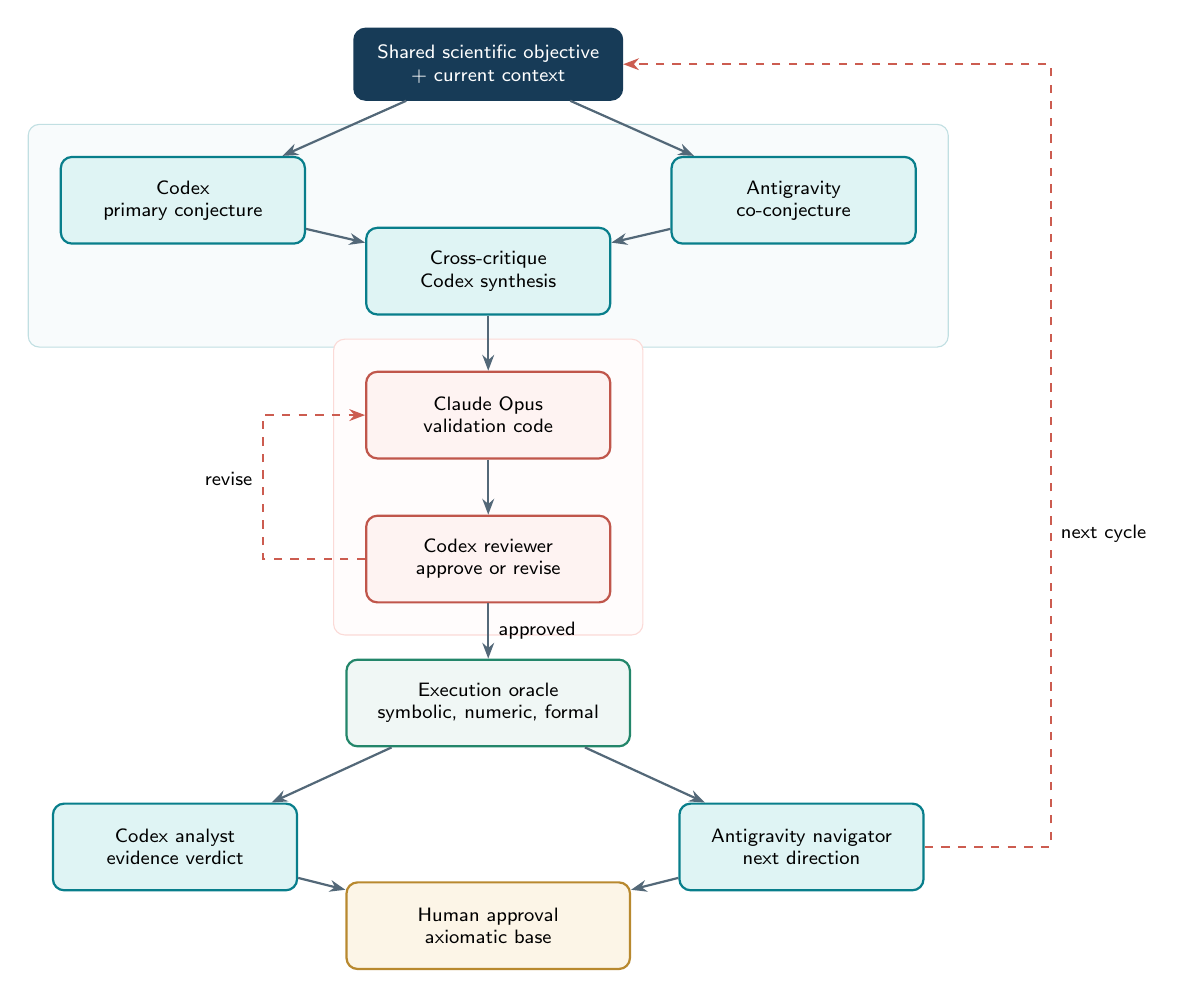
\begin{tikzpicture}[
  node distance=7mm and 6mm,
  font=\sffamily\scriptsize,
  objective/.style={rounded corners,draw=navy,fill=navy,text=white,thick,align=center,minimum width=34mm,minimum height=9mm},
  model/.style={rounded corners,draw=tealblue,fill=cyanlite,thick,align=center,minimum width=31mm,minimum height=11mm},
  review/.style={rounded corners,draw=coral!80!black,fill=coral!8,thick,align=center,minimum width=31mm,minimum height=11mm},
  engine/.style={rounded corners,draw=green,fill=green!7,thick,align=center,minimum width=36mm,minimum height=11mm},
  human/.style={rounded corners,draw=gold!80!black,fill=gold!12,thick,align=center,minimum width=36mm,minimum height=11mm},
  arr/.style={-{Stealth[length=2mm]},thick,draw=slate},
  loop/.style={-{Stealth[length=2mm]},thick,dashed,draw=coral!85!black}
]
\node[objective] (goal) {Shared scientific objective\\+ current context};
\node[model,below left=of goal] (codexconj) {Codex\\primary conjecture};
\node[model,below right=of goal] (agyconj) {Antigravity\\co-conjecture};
\node[model,below=16mm of goal] (synth) {Cross-critique\\Codex synthesis};
\node[review,below=of synth] (claude) {Claude Opus\\validation code};
\node[review,below=of claude] (reviewer) {Codex reviewer\\approve or revise};
\node[engine,below=of reviewer] (oracle) {Execution oracle\\symbolic, numeric, formal};
\node[model,below left=of oracle] (analyst) {Codex analyst\\evidence verdict};
\node[model,below right=of oracle] (navigator) {Antigravity navigator\\next direction};
\node[human,below=17mm of oracle] (gate) {Human approval\\axiomatic base};

\draw[arr] (goal)--(codexconj);
\draw[arr] (goal)--(agyconj);
\draw[arr] (codexconj)--(synth);
\draw[arr] (agyconj)--(synth);
\draw[arr] (synth)--(claude);
\draw[arr] (claude)--(reviewer);
\draw[arr] (reviewer)--node[right]{approved}(oracle);
\draw[loop] (reviewer.west) -- ++(-13mm,0) |- node[pos=.28,left]{revise} (claude.west);
\draw[arr] (oracle)--(analyst);
\draw[arr] (oracle)--(navigator);
\draw[arr] (analyst)--(gate);
\draw[arr] (navigator)--(gate);
\draw[loop] (navigator.east) -- ++(16mm,0) |- node[pos=.20,right]{next cycle} (goal.east);

\begin{scope}[on background layer]
\node[fit=(codexconj)(agyconj)(synth),fill=tealblue!3,draw=tealblue!25,rounded corners,inner sep=4mm] {};
\node[fit=(claude)(reviewer),fill=coral!2,draw=coral!25,rounded corners,inner sep=4mm] {};
\end{scope}
\end{tikzpicture}
\end{center}

\begin{darkbox}
\textbf{Role separation is the central control.}
Codex leads conjecture, synthesis, code review and evidence analysis.
Antigravity contributes an independent conjecture and maintains research direction.
Claude authors and revises validation code. Deterministic engines, not model consensus,
produce the evidence.
\end{darkbox}

\subsection*{Interfaces and deployment}

\begin{tabularx}{\textwidth}{@{}>{\bfseries\color{navy}}p{3.2cm} Y@{}}
\toprule
Layer & Current implementation \\
\midrule
Interaction & Browser interface, command-line subprocess API and MCP tools for agents \\
Orchestration & Asynchronous Python pipeline with progress, timeouts, fallbacks and detached jobs \\
Models & Subscription-authenticated Codex, Claude Code and Antigravity CLIs; optional API providers \\
Execution & Local Python and optional remote Linux worker; engine-specific routing \\
Persistence & Reports, cycle state, research branches, benchmark results and human approval \\
Security posture & Credentials remain in local configuration; private execution is supported; enterprise controls remain a hardening priority \\
\bottomrule
\end{tabularx}

\newpage
\section*{The core algorithm}

\begin{plainbox}
\textbf{Inputs:} shared objective $G$, established context $K$, current direction $D$,
maximum code revisions $R$, execution policy $O$.

\medskip
\ttfamily\small
1.\quad $p_c \leftarrow \mathrm{Codex.propose}(G,K,D)$\\
2.\quad $p_a \leftarrow \mathrm{Antigravity.propose}(G,K,D)$ \hfill [parallel]\\
3.\quad $q_c \leftarrow \mathrm{Codex.critique}(p_a)$;\quad
             $q_a \leftarrow \mathrm{Antigravity.critique}(p_c)$\\
4.\quad $h \leftarrow \mathrm{Codex.synthesize}(G,p_c,p_a,q_c,q_a)$\\
5.\quad $v_0 \leftarrow \mathrm{Claude.translate}(G,h)$\\
6.\quad for $i=0,\ldots,R$:\\
\hspace*{7mm}$r_i \leftarrow \mathrm{Codex.review}(G,h,v_i)$\\
\hspace*{7mm}if $r_i=\mathrm{APPROVED}$: break\\
\hspace*{7mm}$v_{i+1} \leftarrow \mathrm{Claude.revise}(v_i,r_i)$\\
7.\quad $e \leftarrow \mathrm{Oracle.execute}(v_i,O)$\\
8.\quad $s \leftarrow \mathrm{Guard}(v_i,e)$\\
9.\quad $a \leftarrow \mathrm{Codex.analyze}(G,h,v_i,e,s)$\\
10.\quad $n \leftarrow \mathrm{Antigravity.navigate}(G,K,h,a)$\\
11.\quad $\mathrm{HumanGate}(h,v_i,e,a,n)$
\end{plainbox}

\subsection*{Conservative decision semantics}

The orchestration enforces several monotonic constraints:

\begin{itemize}
  \item a crashed validator cannot become \texttt{VALIDATED};
  \item an explicit \texttt{FAIL} cannot be promoted by explanatory prose;
  \item a printed \texttt{PASS} is evidence, not authority;
  \item missing optional engines fail explicitly;
  \item a reviewer can reject circular, unreachable or sampling-only proof logic;
  \item final admission to the axiomatic base requires a human decision.
\end{itemize}

\subsection*{State model}

\begin{center}
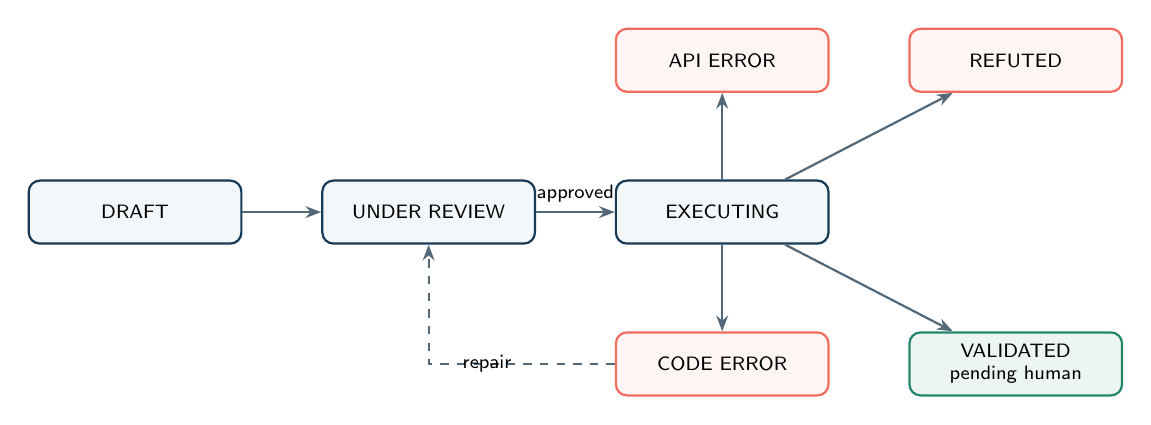
\begin{tikzpicture}[
  font=\sffamily\scriptsize,
  node distance=11mm and 10mm,
  st/.style={rounded corners,draw=navy,fill=mist,thick,minimum width=27mm,minimum height=8mm,align=center},
  ok/.style={rounded corners,draw=green,fill=green!8,thick,minimum width=27mm,minimum height=8mm,align=center},
  fail/.style={rounded corners,draw=coral,fill=coral!7,thick,minimum width=27mm,minimum height=8mm,align=center},
  arr/.style={-{Stealth[length=2mm]},thick,draw=slate}
]
\node[st] (draft) {DRAFT};
\node[st,right=of draft] (review) {UNDER REVIEW};
\node[st,right=of review] (run) {EXECUTING};
\node[ok,below right=of run] (valid) {VALIDATED\\pending human};
\node[fail,above right=of run] (refute) {REFUTED};
\node[fail,below=of run] (codeerr) {CODE ERROR};
\node[fail,above=of run] (apierr) {API ERROR};

\draw[arr] (draft)--(review);
\draw[arr] (review)--node[above]{approved}(run);
\draw[arr] (run)--(valid);
\draw[arr] (run)--(refute);
\draw[arr] (run)--(codeerr);
\draw[arr] (run)--(apierr);
\draw[arr,dashed] (codeerr.west) -| node[pos=.25,left]{repair} (review.south);
\end{tikzpicture}
\end{center}

\begin{keybox}
\textbf{Interpretation boundary.} In ASTRA, \texttt{VALIDATED} means supported by
the recorded validator, execution and assumptions. It does not mean absolute truth.
The evidence remains open to stronger proof, independent replication and expert review.
\end{keybox}

\newpage
\section*{Scientific engine and extension model}

\subsection*{Oracle portfolio}

\begin{tabularx}{\textwidth}{@{}>{\bfseries\color{navy}}p{3.1cm} p{4.1cm} Y@{}}
\toprule
Engine class & Examples & Validation role \\
\midrule
Symbolic & SymPy, SageMath, Maxima & Exact simplification, identities, derivatives, algebraic residuals \\
Logic / proof & Z3, Lean 4 + Mathlib & Counterexample search, satisfiability, kernel-checked theorems \\
Numerical & NumPy, SciPy, mpmath, QuTiP & ODEs, high-precision checks, quantum systems, sweeps \\
Domain packages & EinsteinPy, fluids, Pint & Curvature, fluid models, units and physical consistency \\
Independent CAS & Mathematica bridge, Cadabra & Cross-engine validation, tensor algebra, notebook workflows \\
Internal software & GR\_python, pyWarpFactory, warp-bubble optimization & Reuse of proprietary or project-specific research capabilities \\
\bottomrule
\end{tabularx}

\subsection*{Extension contract}

Any scientific package can become part of the oracle when a validator:

\begin{enumerate}
  \item declares reproducible inputs, versions and assumptions;
  \item imports the package in the selected environment;
  \item computes a quantity that discriminates the claim from its negation;
  \item exposes exact output, errors and tolerances;
  \item includes reachable failure behavior;
  \item preserves the script and result for review.
\end{enumerate}

\subsection*{Agent control through MCP}

ASTRA exposes operations for direct execution, complete cycles, progress probes,
detached jobs, job polling and remote-worker status. A conversational agent can
therefore plan a test and invoke ASTRA without manually copying code, while ASTRA
retains the evidence and decision semantics.

\begin{plainbox}
\textbf{Illustrative client instruction:}\\
``Formulate two competing explanations for this curvature result. Use ASTRA to
construct a validator with an exact symbolic leg and an independent numerical leg.
Do not accept a printed PASS until the code, residuals and assumptions have been
reviewed.''
\end{plainbox}

\subsection*{Enterprise productization priorities}

\begin{multicols}{2}
\begin{itemize}
  \item workspace authentication and role-based access;
  \item signed evidence bundles and immutable audit metadata;
  \item dependency and container pinning;
  \item job isolation and compute quotas;
  \item private model and on-premise connectors;
  \item team review queues and approval policy;
  \item observability, cost and latency dashboards;
  \item benchmark governance and release qualification.
\end{itemize}
\end{multicols}

\newpage
\section*{Commercialization roadmap}

\begin{tabularx}{\textwidth}{@{}>{\bfseries\color{navy}}p{2.5cm} p{4.0cm} Y@{}}
\toprule
Phase & Product objective & Evidence required before advancing \\
\midrule
Now & Operational multi-model research loop and scientific oracle & Repeated benchmark passes; documented end-to-end cycles; reproducible local installation \\
\addlinespace
Pilot hardening & Deploy with a small number of design partners & Measured time-to-evidence, reviewer correction value, reproduction rate and expert satisfaction \\
\addlinespace
Team product & Shared projects, governed approvals and scalable jobs & Repeat use, retained teams, security acceptance and clear economic buyer \\
\addlinespace
Vertical modules & Domain-specific validators, packages and benchmark suites & Superior outcomes in selected high-value workflows \\
\addlinespace
Platform expansion & Private deployment, partner engines and model marketplace & Reliable operations, integration demand and sustainable unit economics \\
\bottomrule
\end{tabularx}

\subsection*{Near-term capital and partnership priorities}

\begin{enumerate}
  \item \textbf{Product engineering:} packaging, secure execution, observability,
  collaboration and evidence management.
  \item \textbf{Scientific calibration:} adversarial benchmarks, false-acceptance
  measurement and expert-reviewed domain suites.
  \item \textbf{Design partnerships:} two or three workflows with high verification
  cost and measurable research-cycle value.
  \item \textbf{Distribution:} model, compute, scientific-software and research
  institution integrations.
\end{enumerate}

\subsection*{Risks and mitigations}

\begin{riskbox}
\begin{tabularx}{\textwidth}{@{}>{\bfseries}p{3.1cm} Y Y@{}}
Risk & Why it matters & Mitigation direction \\
\midrule
Validator mismatch & Code may test a weaker or different claim & Independent code review, human gate, benchmarked failure patterns \\
Model latency and quota & Maximum-quality cycles can take minutes & Phase budgets, fallbacks, caching, fast and deep profiles \\
False confidence & Users may overread \texttt{VALIDATED} & Explicit semantics, evidence display, independent engines, approval policy \\
Scientific breadth & No system is expert in every domain & Vertical focus, package adapters, domain reviewers and scoped claims \\
Enterprise security & Generated code executes with real resources & Isolation, allowlists, containers, credentials policy and audit logs \\
Go-to-market diffusion & ``Science'' is too broad as an initial segment & Start with measurable design-partner workflows and a specific buyer \\
\end{tabularx}
\end{riskbox}

\subsection*{The next proof points}

\begin{itemize}
  \item demonstrate lower false-acceptance rates than a single-model baseline;
  \item reproduce partner results across a second environment or engine;
  \item quantify expert time saved per accepted or refuted claim;
  \item identify one vertical where ASTRA becomes a paid part of the weekly R\&D workflow.
\end{itemize}

\newpage
\section*{Engagement proposal}

\begin{darkbox}
{\Large\bfseries The product thesis in one sentence}\par
\vspace{2mm}
ASTRA is the verification and coordination layer that allows organizations to use
frontier AI in scientific work while preserving falsifiability, reproducibility and
human control.
\end{darkbox}

\subsection*{For a prospective client}

Select one consequential workflow with:

\begin{itemize}
  \item a clear scientific decision and current baseline process;
  \item existing code, equations, simulations or internal packages;
  \item measurable verification effort or rework;
  \item an expert who can judge whether ASTRA preserves the real claim.
\end{itemize}

A pilot should compare baseline and ASTRA-assisted work on time-to-evidence,
reproducibility, review effort and false acceptance.

\subsection*{For an investor or VC}

The immediate diligence questions are concrete:

\begin{enumerate}
  \item Does independent review materially improve generated validators?
  \item Which customer segment has the highest cost of unverifiable AI output?
  \item Can the evidence architecture become a repeatable team workflow?
  \item Which data, adapters and calibration assets compound with usage?
  \item Can private deployment and scientific specialization support durable economics?
\end{enumerate}

\subsection*{For a strategic partner}

ASTRA can provide a governed research workflow around:

\begin{itemize}
  \item frontier models that need credible scientific demonstrations;
  \item compute platforms that want traceable high-value workloads;
  \item scientific-software vendors seeking agent-native interfaces;
  \item research organizations building reproducible AI-assisted methods.
\end{itemize}

\begin{keybox}
\textbf{Proposed next step.} Define a 4--8 week design-partner study around one
scientific workflow, one baseline, one reproducibility target and an agreed set of
acceptance metrics. The goal is not a demo; it is evidence that ASTRA changes a real
R\&D decision.
\end{keybox}

\vfill
\begin{center}
{\Large\bfseries\color{navy}ASTRA}\par
\vspace{2mm}
{\large\color{tealblue}From plausible answers to reviewable evidence.}\par
\vspace{8mm}
{\small Nelson Bolívar | Founder and Lead Architect | Astrum Drive}\par
{\small Investor, client and strategic partner discussions | July 2026}
\end{center}

\end{document}
